\documentclass[a4paper,11pt]{article}
\usepackage[utf8]{inputenc}
\usepackage[T1]{fontenc}
\usepackage[brazilian]{babel}
\usepackage[margin=2.2cm]{geometry}
\usepackage{amsmath}
\usepackage{graphicx}
\usepackage{booktabs}
\usepackage{float}
\usepackage{caption}
\usepackage{subcaption}
\usepackage{hyperref}

\graphicspath{{../figuras/}}

\title{F056 -- Lista de Exercícios: Simulação de Detectores com Geant4\\
\large Calorímetro de amostragem do exemplo B4a}
\author{Guilherme de Medeiros}
\date{\today}

\begin{document}

\maketitle

\noindent Todas as simulações foram feitas com o Geant4 11.4.3 (ambiente conda \texttt{g4env},
lista de física \texttt{FTFP\_BERT}, a mesma do exemplo). Código, macros e instruções de execução
estão no \texttt{README.md} do diretório \texttt{lista\_geant4/}. As modificações no B4a estão
listadas na Seção~\ref{sec:mod} e no arquivo \texttt{modificacoes\_B4a.diff}.

%=====================================================================
\section{Exercício 1 -- O exemplo B4a}
%=====================================================================

\subsection{(a) Descrição do detector}

O B4a simula um \textbf{calorímetro de amostragem} (\emph{sampling calorimeter}) eletromagnético:
camadas alternadas de um material denso e passivo, que provoca e desenvolve o chuveiro, e de um
material ativo, onde a energia depositada seria medida.

\begin{itemize}
  \item \textbf{Absorvedor}: chumbo (\texttt{G4\_Pb}, $\rho = 11{,}35$~g/cm$^3$). Alto $Z$, comprimento de radiação
    curto ($X_0 = 5{,}61$~mm): é onde o chuveiro se desenvolve e onde fica a maior parte da energia.
    Não é lido, é passivo.
  \item \textbf{Meio ativo (\emph{gap})}: argônio líquido (\texttt{liquidArgon}, definido à mão com
    $Z=18$, $A = 39{,}95$~g/mol, $\rho = 1{,}39$~g/cm$^3$, porque o argônio do NIST é gás). Num detector
    real as partículas carregadas ionizam o argônio e a carga é coletada; a energia nele é a ``medida''.
  \item \textbf{Mundo e mãe do calorímetro}: \texttt{Galactic} (vácuo, $\rho \approx 10^{-25}$~g/cm$^3$).
\end{itemize}

\noindent Geometria (parâmetros em \texttt{DetectorConstruction::DefineVolumes()}):
\begin{itemize}
  \item 10 camadas (\texttt{nofLayers}), cada uma com 10~mm de chumbo (\texttt{absoThickness}) seguidos de
    5~mm de argônio líquido (\texttt{gapThickness}): camada de 15~mm;
  \item seção transversal quadrada de $10 \times 10$~cm$^2$ (\texttt{calorSizeXY});
  \item comprimento total de $10 \times 15 = 150$~mm; o mundo é 20\% maior ($12 \times 12 \times 18$~cm$^3$);
  \item as camadas são réplicas (\texttt{G4PVReplica}) ao longo de $z$ dentro do volume \texttt{Calorimeter};
    hierarquia: \texttt{World} $\rightarrow$ \texttt{Calorimeter} $\rightarrow$ \texttt{Layer} (×10) $\rightarrow$ \texttt{Abso} e \texttt{Gap};
  \item em unidades físicas: $10\times(10/5{,}61 + 5/140{,}6) = 18{,}2\,X_0$ e
    $10\times(10/182{,}5 + 5/860{,}8) = 0{,}61\,\lambda_I$ (valores de $X_0$ e $\lambda_I$ impressos pelo próprio
    Geant4, \texttt{G4Material::GetRadlen()} e \texttt{GetNuclearInterLength()}).
\end{itemize}

\noindent O feixe (\texttt{PrimaryGeneratorAction}) é um \texttt{G4ParticleGun} com um e$^-$ de 300~MeV por padrão,
saindo de $(0, 0, -9~\text{cm})$ (face do mundo) na direção $+z$, ou seja, entrando no centro da face do calorímetro.
A energia depositada e o comprimento de traço no absorvedor e no gap são somados passo a passo no
\texttt{SteppingAction} e gravados por evento (ntuple \texttt{B4}) no \texttt{EventAction}/\texttt{RunAction}.
Existe ainda um campo magnético uniforme opcional (nulo por padrão, \texttt{/globalField/setValue}).

\noindent\textbf{Onde estão as informações:}
\texttt{src/DetectorConstruction.cc} (materiais em \texttt{DefineMaterials()}, dimensões e volumes em
\texttt{DefineVolumes()}), \texttt{include/DetectorConstruction.hh} (descrição da geometria no comentário da classe),
\texttt{src/PrimaryGeneratorAction.cc} (feixe), \texttt{exampleB4a.cc} (lista de física \texttt{FTFP\_BERT})
e \texttt{src/SteppingAction.cc} / \texttt{src/EventAction.cc} (o que é registrado).

\subsection{(b) Elétron, próton e alfa de 10 GeV no chumbo}

As figuras foram feitas com a macro \texttt{macros/figura.mac} (driver \texttt{TSG\_OFFSCREEN}, que grava o PNG
sem abrir janela; o Geant4 instalado também tem o driver \texttt{OGL} do enunciado, mas não o usei). Cada figura mostra 1 evento. Como 1 evento hadrônico
não é representativo, fiz também figuras com 20 eventos sobrepostos para o próton e o alfa. Para ter números,
rodei 500 eventos de cada caso sem visualização (Tabela~\ref{tab:ex1}).

\begin{figure}[H]
  \centering
  \begin{subfigure}{0.49\textwidth}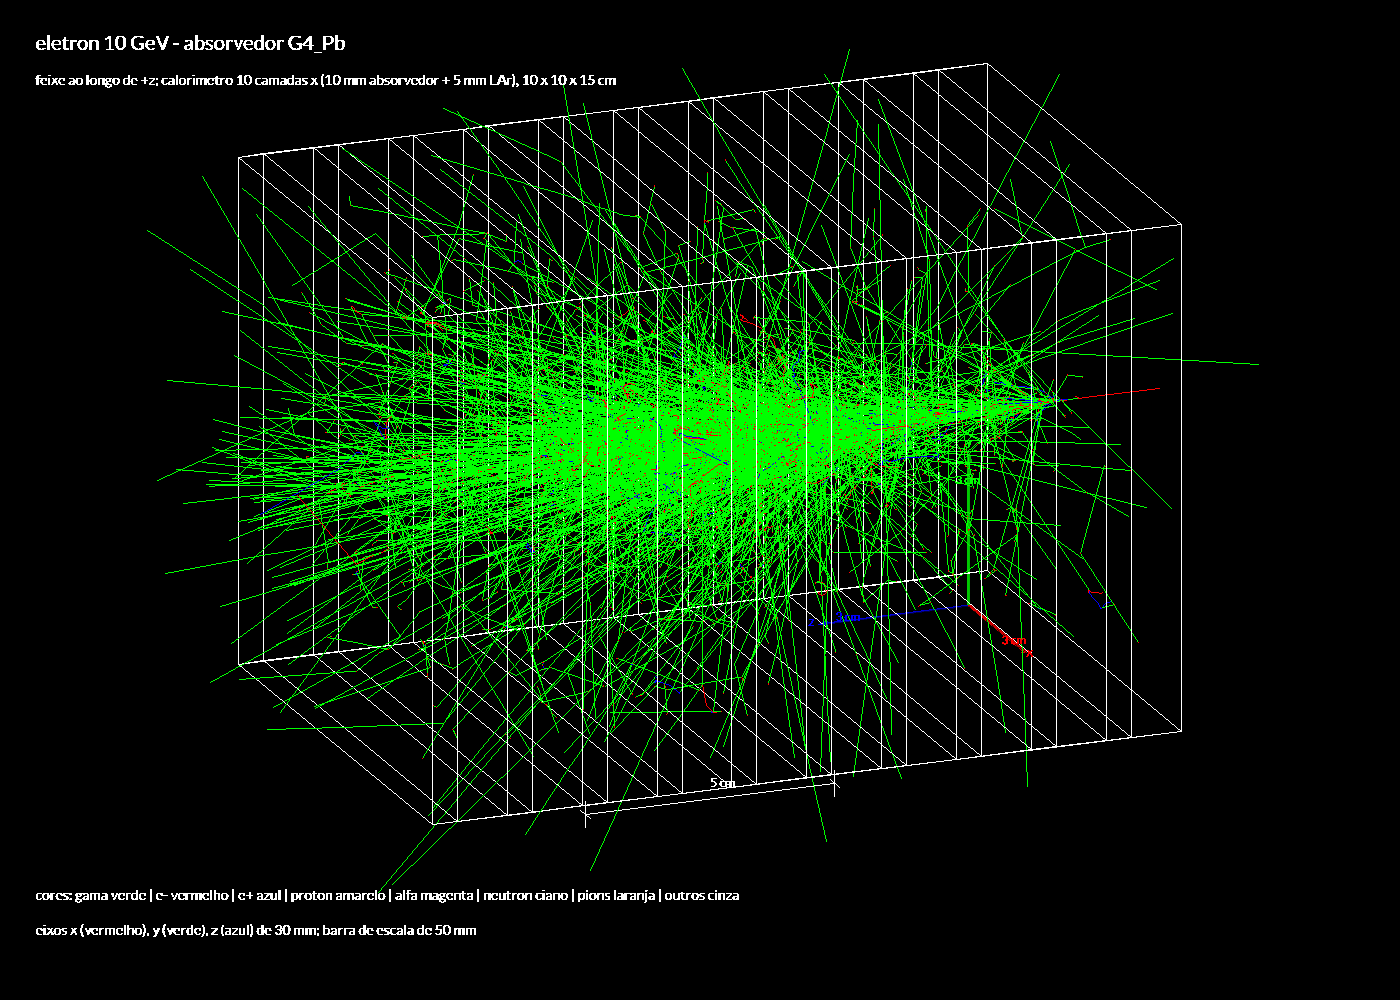
\includegraphics[width=\textwidth]{eletron_10GeV_Pb.png}\caption{e$^-$, 1 evento}\end{subfigure}
  \begin{subfigure}{0.49\textwidth}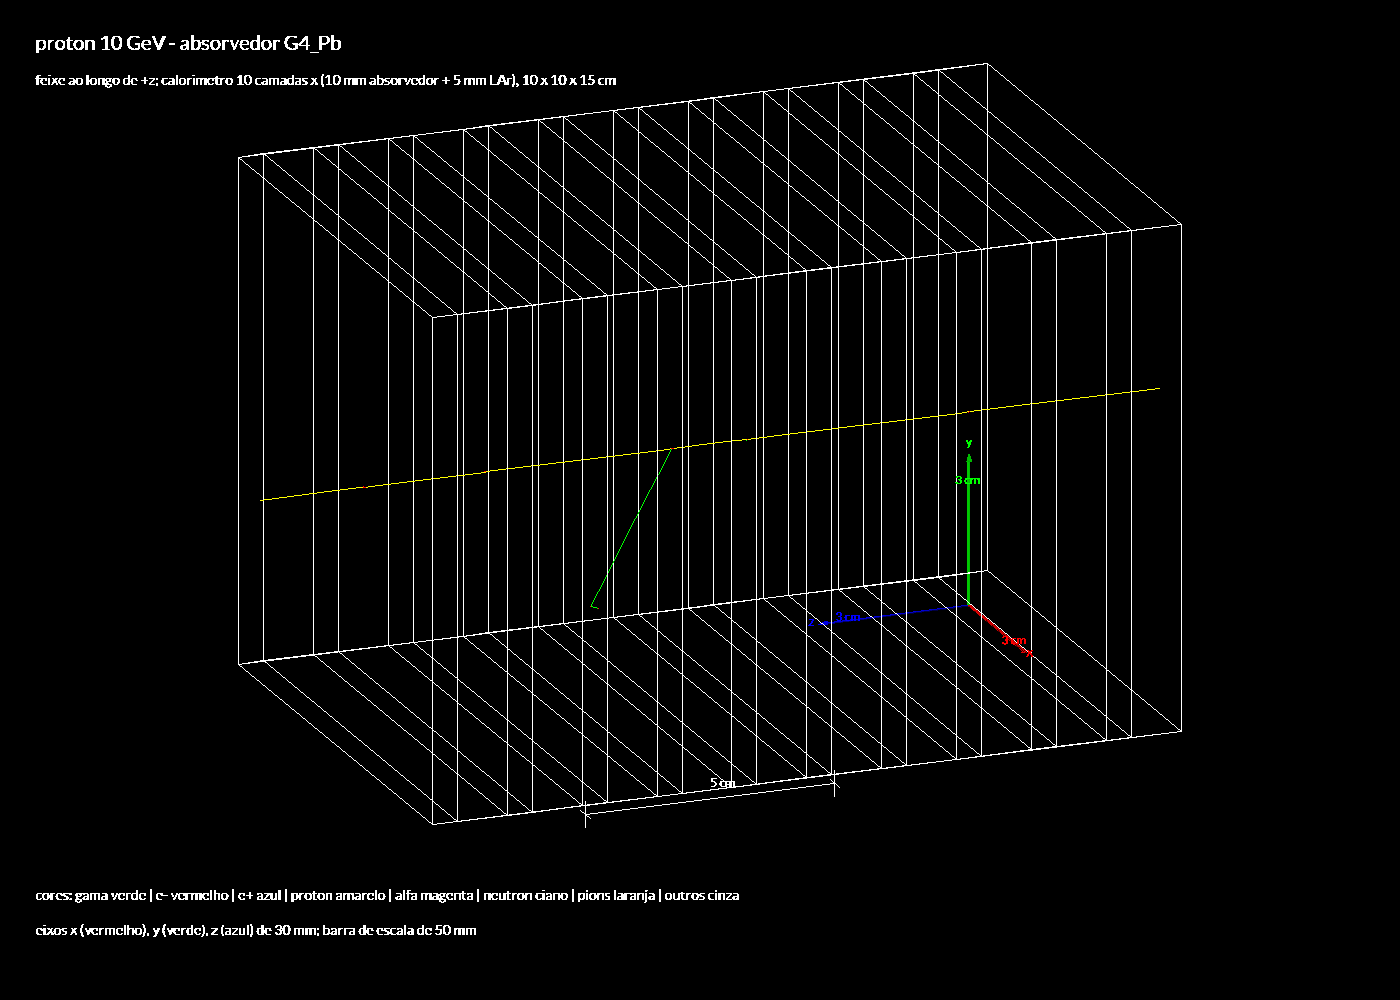
\includegraphics[width=\textwidth]{proton_10GeV_Pb.png}\caption{próton, 1 evento}\end{subfigure}
  \begin{subfigure}{0.49\textwidth}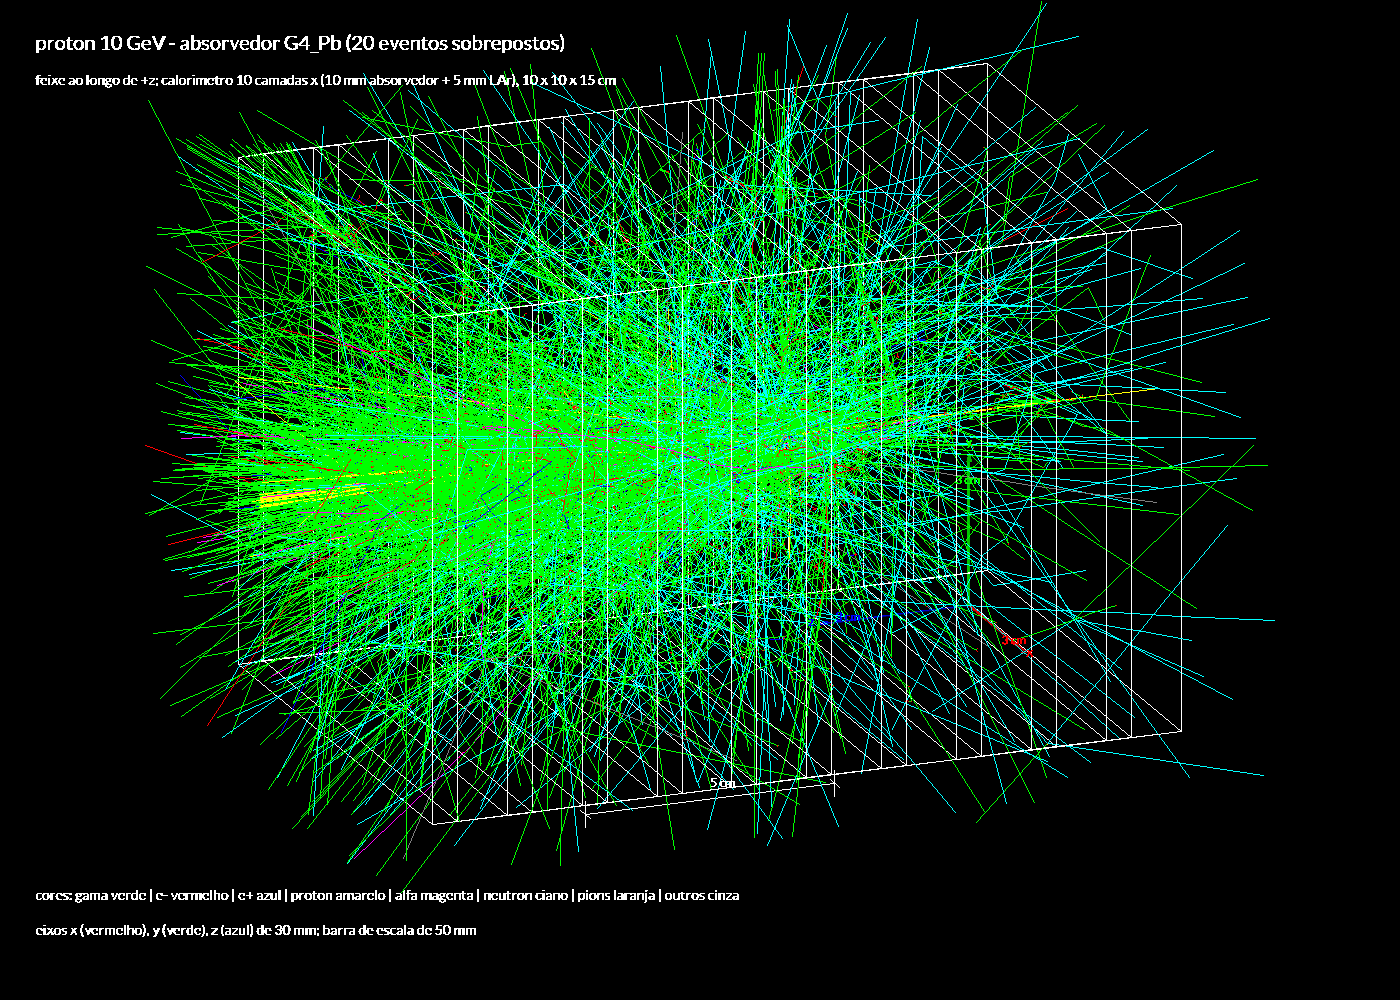
\includegraphics[width=\textwidth]{proton_10GeV_Pb_20eventos.png}\caption{próton, 20 eventos}\end{subfigure}
  \begin{subfigure}{0.49\textwidth}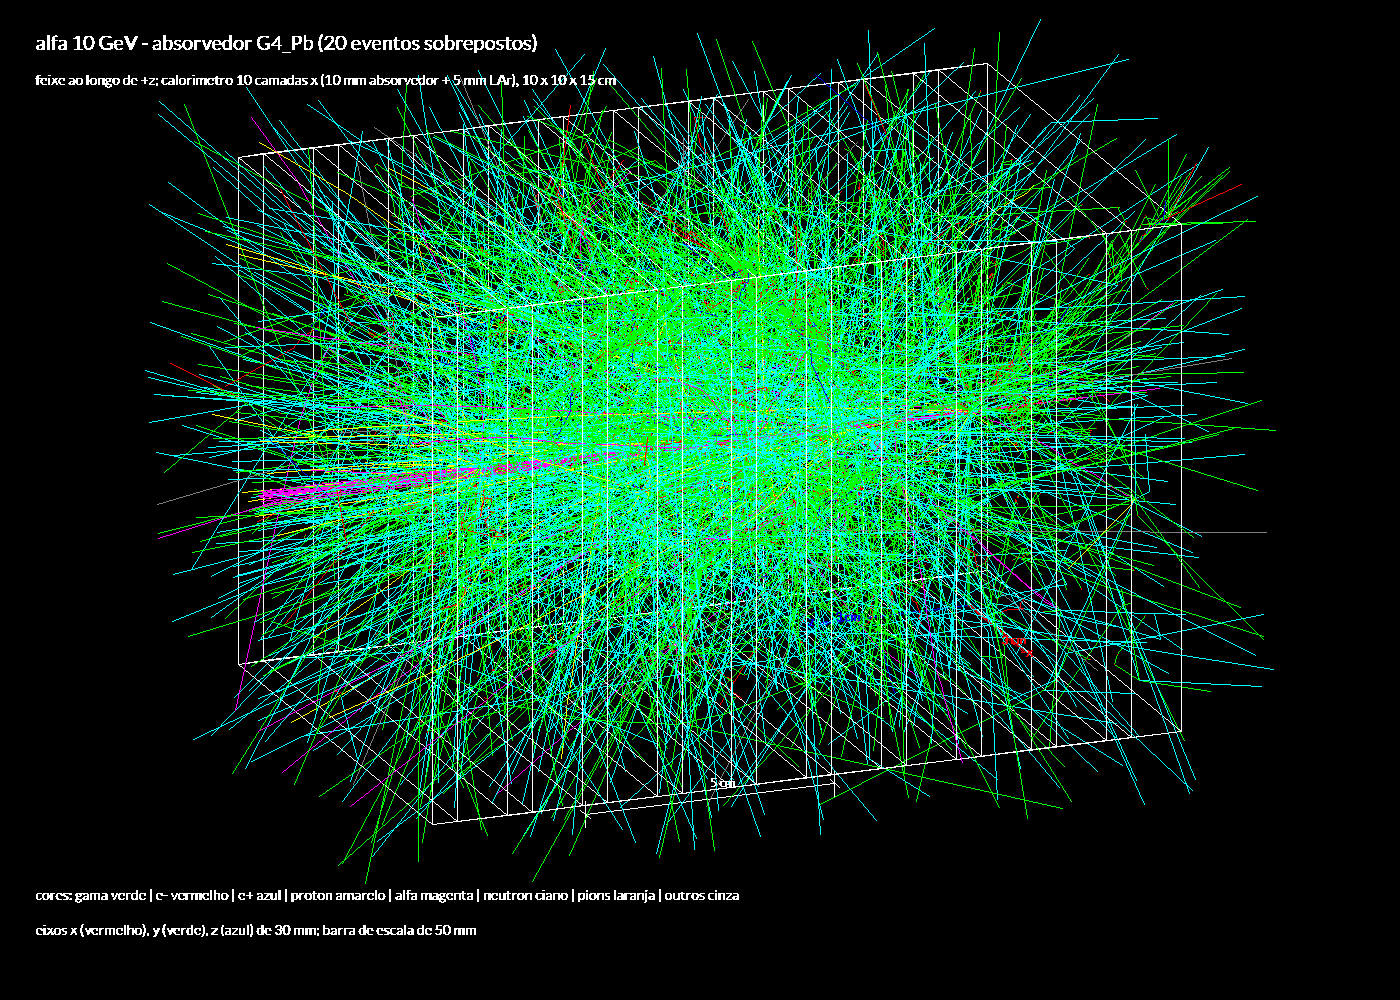
\includegraphics[width=\textwidth]{alfa_10GeV_Pb_20eventos.png}\caption{alfa, 20 eventos}\end{subfigure}
  \caption{Partículas de 10 GeV no calorímetro Pb/LAr (feixe da esquerda para a direita, ao longo de $+z$).
  Cores: $\gamma$ verde, e$^-$ vermelho, e$^+$ azul, próton amarelo, alfa magenta, nêutron ciano, píons laranja,
  outros cinza. Os eixos têm 30~mm e a barra de escala, 50~mm. A figura do alfa com 1 evento está em
  \texttt{figuras/alfa\_10GeV\_Pb.png}.}
  \label{fig:pb}
\end{figure}

\begin{table}[H]
\centering
\caption{Energia depositada (500 eventos por caso, 10 GeV). ``Sem chuveiro'' é a fração de eventos com
$E_{\text{tot}} < 1{,}5\times$ a posição do pico de MIP, ou seja, que atravessaram só ionizando.}
\label{tab:ex1}
\begin{tabular}{llrrrrrr}
\toprule
absorvedor & partícula & $\langle E_\text{abs}\rangle$ (MeV) & $\langle E_\text{gap}\rangle$ (MeV) &
$\langle E_\text{tot}\rangle/E_0$ & rms$/E_0$ & pico MIP (MeV) & sem chuveiro \\
\midrule
Pb   & e$^-$  & 8881 & 489  & 0,937  & 0,021  & --    & --   \\
Pb   & próton & 1306 & 95   & 0,140  & 0,162  & 144   & 0,51 \\
Pb   & alfa   & 1374 & 101  & 0,148  & 0,112  & 554   & 0,50 \\
água & e$^-$  & 34   & 20   & 0,0054 & 0,0027 & --    & --   \\
água & próton & 57   & 32   & 0,0089 & 0,016  & 28    & 0,77 \\
água & alfa   & 107  & 58   & 0,0166 & 0,011  & 118   & 0,80 \\
\bottomrule
\end{tabular}
\end{table}

\begin{figure}[H]
  \centering
  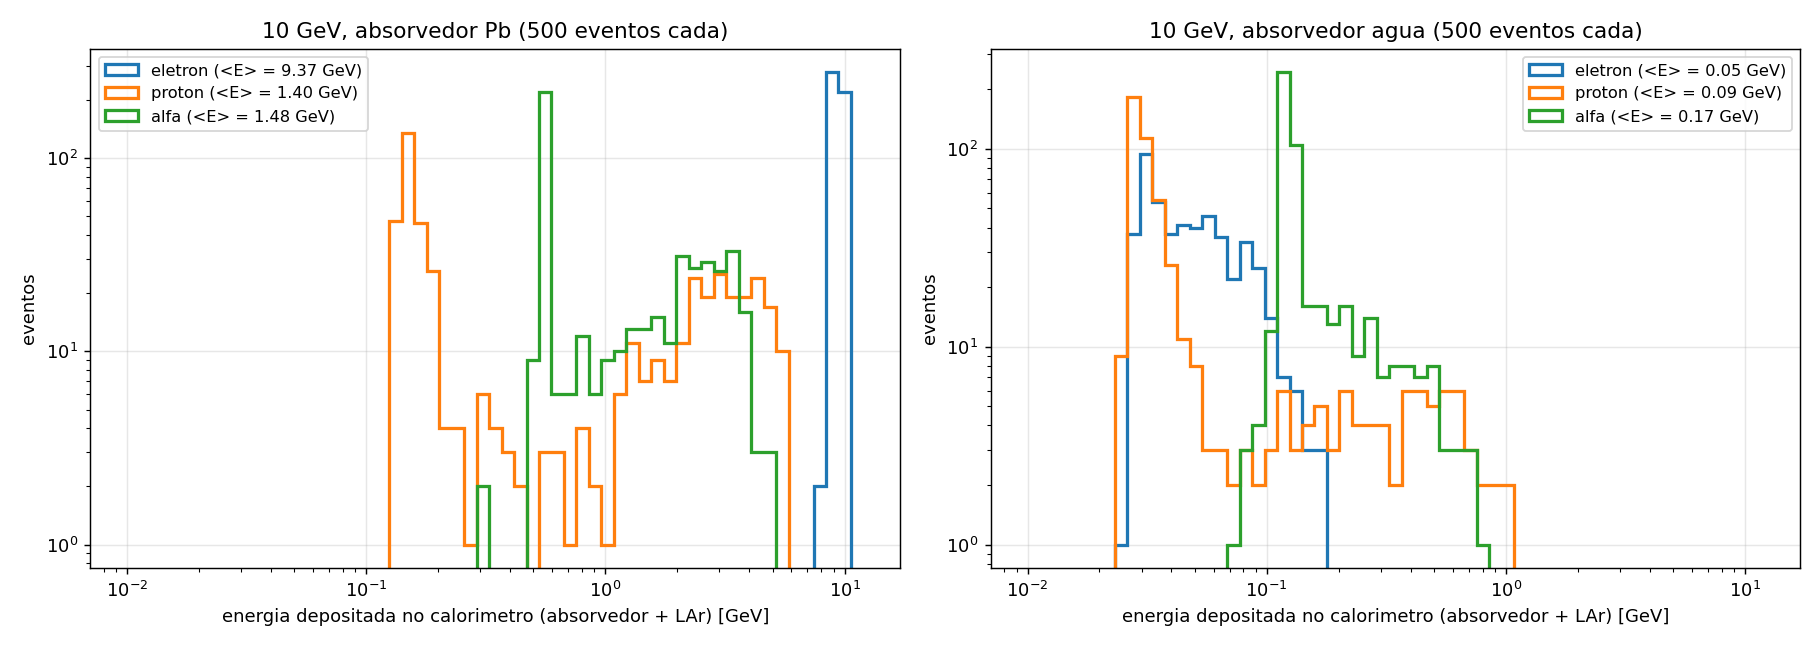
\includegraphics[width=\textwidth]{ex1_energia_depositada.png}
  \caption{Distribuição da energia depositada no calorímetro (absorvedor + LAr) por evento, para 500 partículas
  de 10 GeV de cada tipo, com absorvedor de chumbo (esquerda) e de água (direita). Eixos em escala log.}
  \label{fig:edep}
\end{figure}

\noindent\textbf{Elétron.} Desenvolve um chuveiro \textbf{eletromagnético} completo: bremsstrahlung e produção de
pares se alternam a cada $\sim X_0$, gerando milhares de fótons (verde) e e$^\pm$ de baixa energia. O chuveiro é
compacto (alguns cm de raio), tem máximo por volta de $6\,X_0$ (3ª--4ª camada) e o calorímetro (18~$X_0$) contém
\textbf{94\%} da energia, com flutuação pequena (rms de 2\%). É o caso para o qual o calorímetro foi feito.

\noindent\textbf{Próton.} O calorímetro tem só $0{,}61\,\lambda_I$, então a probabilidade de o próton atravessar sem
interação inelástica é $e^{-0{,}61} \approx 0{,}55$. Na simulação, 51\% dos eventos são \textbf{MIP}: o próton
atravessa em linha reta depositando só $\approx 144$~MeV por ionização (pico estreito da Fig.~\ref{fig:edep}).
Quando interage, faz um chuveiro \textbf{hadrônico}: píons, prótons e muitos nêutrons (ciano) da quebra nuclear,
fótons de $\pi^0 \to \gamma\gamma$ (componente EM) e da desexcitação nuclear. Esse chuveiro é muito mais largo e longo
que o EM e não cabe no calorímetro. Em média só \textbf{14\%} da energia fica, com flutuação enorme (rms de 16\% de $E_0$,
maior que a média). Parte da energia vai para quebrar núcleos e para nêutrons lentos, e não aparece como ionização.

\noindent\textbf{Alfa.} O pico de MIP fica em 554~MeV, $\approx 3{,}9\times$ o do próton, porque $dE/dx \propto Z^2$
($Z=2$). A seção de choque nuclear do alfa é maior que a do próton, então ele interage mais, mas o alfa também se
\textbf{fragmenta} (em p, n, d, $^3$He) em colisões periféricas, e esses fragmentos continuam quase como MIPs e
depositam menos que o próprio alfa. Por isso a fração ``sem chuveiro'' (0,50) é parecida com a do próton, e não
menor. Os chuveiros do alfa têm mais fragmentos nucleares e nêutrons. A energia média contida (15\%) é parecida
com a do próton, mas com flutuação menor.

\subsection{(c) Absorvedor de água}

Troquei o material com o comando \texttt{/B4/det/absorberMaterial G4\_WATER} (antes do \texttt{/run/initialize}),
que eu adicionei no \texttt{DetectorConstruction}.

\begin{figure}[H]
  \centering
  \begin{subfigure}{0.32\textwidth}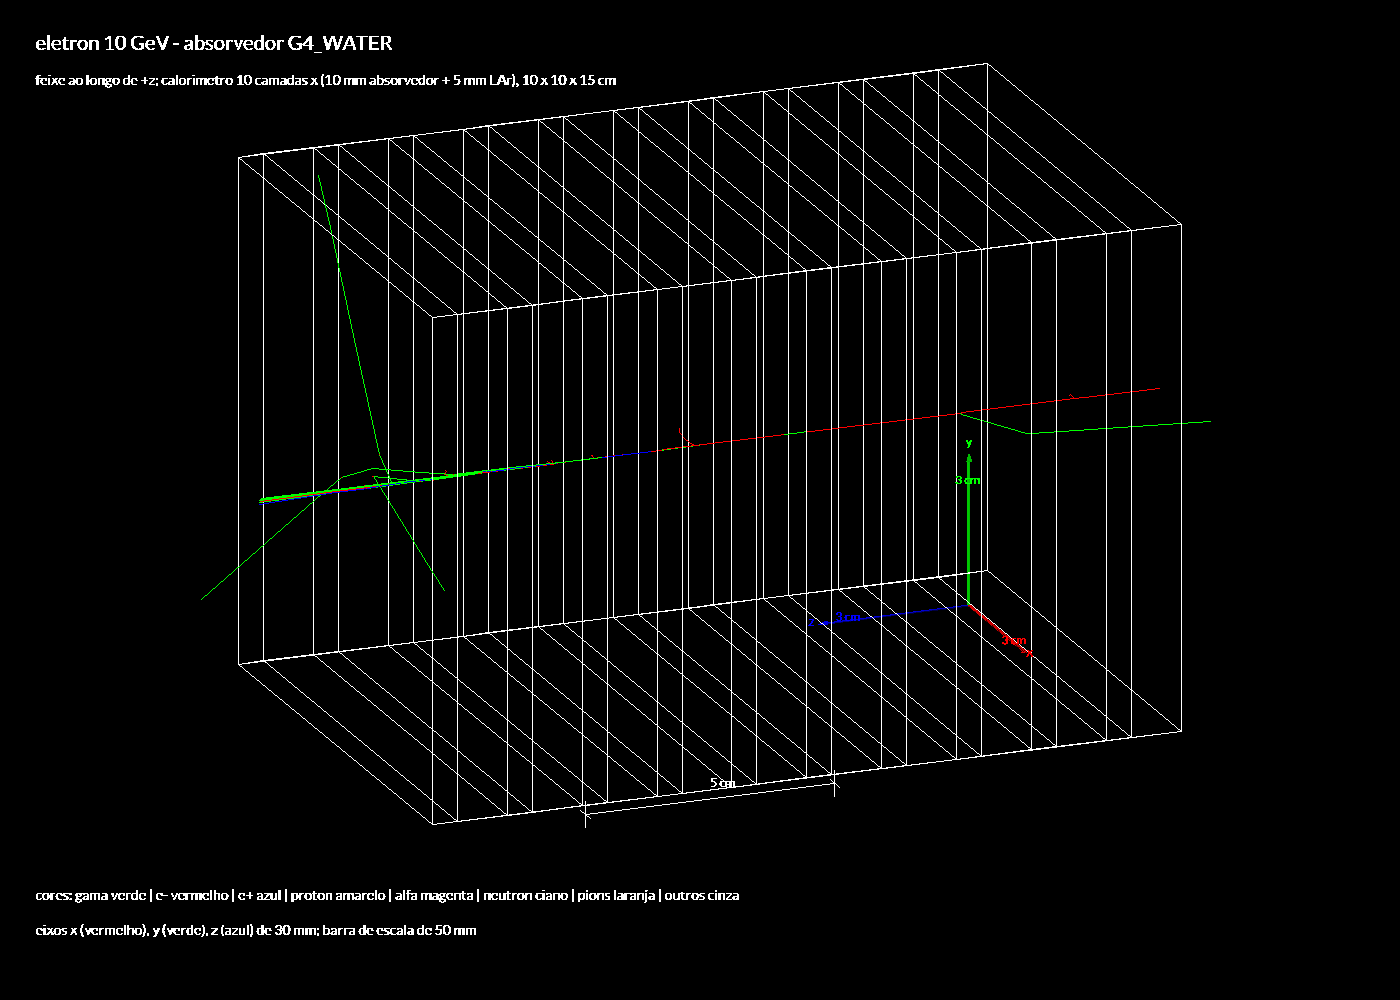
\includegraphics[width=\textwidth]{eletron_10GeV_agua.png}\caption{e$^-$}\end{subfigure}
  \begin{subfigure}{0.32\textwidth}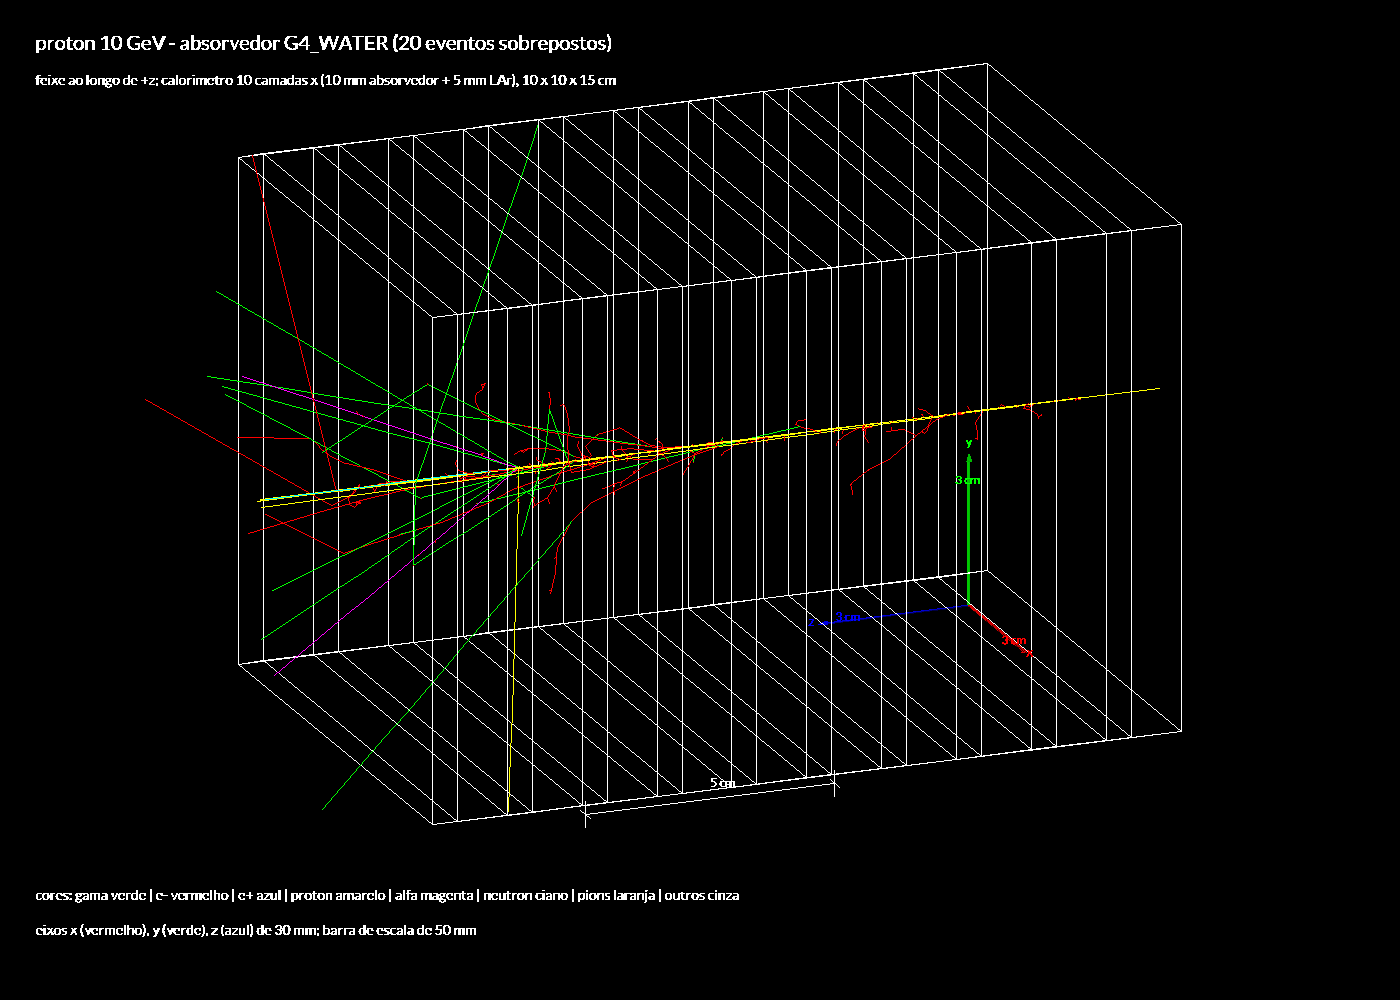
\includegraphics[width=\textwidth]{proton_10GeV_agua_20eventos.png}\caption{próton (20 eventos)}\end{subfigure}
  \begin{subfigure}{0.32\textwidth}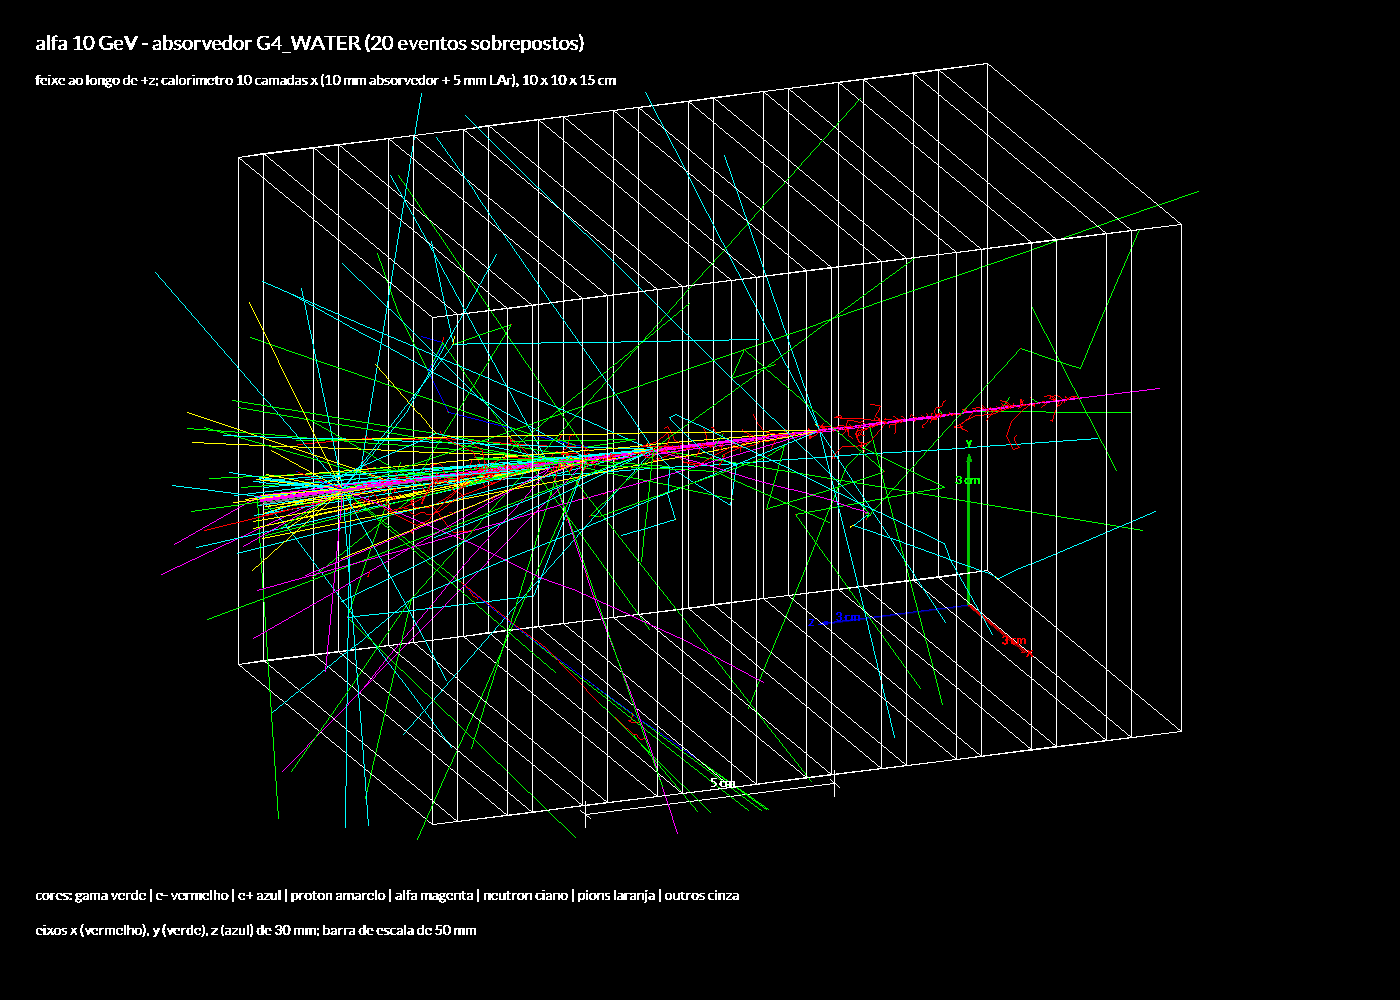
\includegraphics[width=\textwidth]{alfa_10GeV_agua_20eventos.png}\caption{alfa (20 eventos)}\end{subfigure}
  \caption{Mesmas partículas com absorvedor de água (10 mm de água + 5 mm de LAr por camada). As figuras de 1 evento
  do próton e do alfa estão em \texttt{figuras/}.}
\end{figure}

\begin{table}[H]
\centering
\caption{Comprimento de radiação e de interação nuclear (Geant4) e espessura total do calorímetro.}
\begin{tabular}{lrrrr}
\toprule
material & $\rho$ (g/cm$^3$) & $X_0$ (mm) & $\lambda_I$ (mm) & \\
\midrule
chumbo & 11,35 & 5,61 & 182,5 & \\
água & 1,00 & 360,8 & 753,7 & \\
argônio líquido & 1,39 & 140,6 & 860,8 & \\
\midrule
calorímetro Pb/LAr & & \multicolumn{3}{l}{18,2 $X_0$ \quad 0,61 $\lambda_I$} \\
calorímetro água/LAr & & \multicolumn{3}{l}{0,63 $X_0$ \quad 0,19 $\lambda_I$} \\
\bottomrule
\end{tabular}
\end{table}

\noindent Com água o calorímetro tem só $0{,}63\,X_0$: o elétron mal começa a irradiar. Só alguns fótons de
bremsstrahlung saem pela frente, e o elétron deposita $\approx 54$~MeV (0,5\% de $E_0$), basicamente ionização.
O chuveiro nem começa: precisaria de $\sim 6\,X_0 \approx 2$~m de água para chegar ao máximo. Curiosamente, aqui o
argônio tem mais $X_0$ que a água (5~mm de LAr = 0,036~$X_0$, contra 0,028~$X_0$ de 10~mm de água).

\noindent Para os hádrons, $\lambda_I$ da água (75~cm) é 4× o do chumbo, mas a diferença em gramas é bem menor
($\lambda_I$ em g/cm$^2$ cresce devagar com $A$: 75 g/cm$^2$ na água, 207 g/cm$^2$ no chumbo). O calorímetro de água tem
$0{,}19\,\lambda_I$, então 77--80\% dos prótons e alfas passam sem interagir ($e^{-0{,}19} = 0{,}83$ para o próton).
Os que interagem quase não desenvolvem chuveiro dentro do calorímetro. As deposições são as de MIP
($\approx 28$~MeV para o próton e 118~MeV para o alfa, 4× maior por causa do $Z^2$).

\noindent Resumindo: para chuveiros EM o que importa é $X_0$, que é $\propto A/Z^2$ e por isso muito menor em materiais
pesados (chumbo 64× menor que a água). Para chuveiros hadrônicos o que importa é $\lambda_I$, que depende muito
menos de $Z$ (só 4× entre água e chumbo). Por isso calorímetros EM usam Pb ou W, e mesmo o chumbo com 15~cm
não contém hádrons: para isso são necessários $\sim 1$--2~m de ferro ou cobre (vários $\lambda_I$).

%=====================================================================
\section{Exercício 2 -- Perfil longitudinal do chuveiro EM}
%=====================================================================

\subsection{Modificações no B4a}\label{sec:mod}

\begin{itemize}
  \item \texttt{RunAction}: saída em CSV (\texttt{SetDefaultFileType("csv")}, \texttt{SetFileName("calo\_output")}) e uma
    segunda ntuple, \texttt{CaloHits} (id 1), com as colunas \texttt{Edep\_MeV, Layer, x, y, z} do enunciado, mais
    \texttt{EventID} e \texttt{IsGap} (0 = absorvedor, 1 = LAr). Também liguei \texttt{SetActivation(true)}, para poder
    desligar essa ntuple por macro (\texttt{/analysis/ntuple/setActivation 1 false}) nas rodadas em que ela não
    é necessária.
  \item \texttt{SteppingAction}: um registro por passo com $E_\text{dep}>0$ no absorvedor ou no gap. A camada é
    \texttt{GetReplicaNumber(1)} (0 a 9, conferido) e o número do evento vem de
    \texttt{GetCurrentEvent()->GetEventID()} do \texttt{G4RunManager}.
    Em modo multithread os IDs de evento são únicos entre as threads (conferido: 1000 IDs distintos).
  \item \texttt{DetectorConstruction}: comando \texttt{/B4/det/absorberMaterial} (\texttt{G4GenericMessenger}) para
    trocar o absorvedor sem recompilar, e impressão de $X_0$ e $\lambda_I$ dos materiais.
\end{itemize}

\noindent Simulei 1000 e$^-$ de 10 GeV com cada absorvedor (8 threads, 8 arquivos
\texttt{calo\_output\_nt\_CaloHits\_t*.csv}, $\approx 25$ mil registros por evento no chumbo, 1~GB no total).

\subsection{(a) Programa}

O código-base virou o programa \texttt{perfil\_longitudinal.py} (\texttt{argparse} com os padrões dos arquivos de
entrada de cada material e o diretório de saída). Ele lê os CSV um por vez e já agrega por (evento, camada,
volume), então usa menos de 0,5~GB de memória mesmo com 1~GB de entrada. A Fig.~\ref{fig:base}(a) mostra o resultado
do código-base original.

\subsection{(b) Análise crítica: média por registro}

\begin{figure}[H]
  \centering
  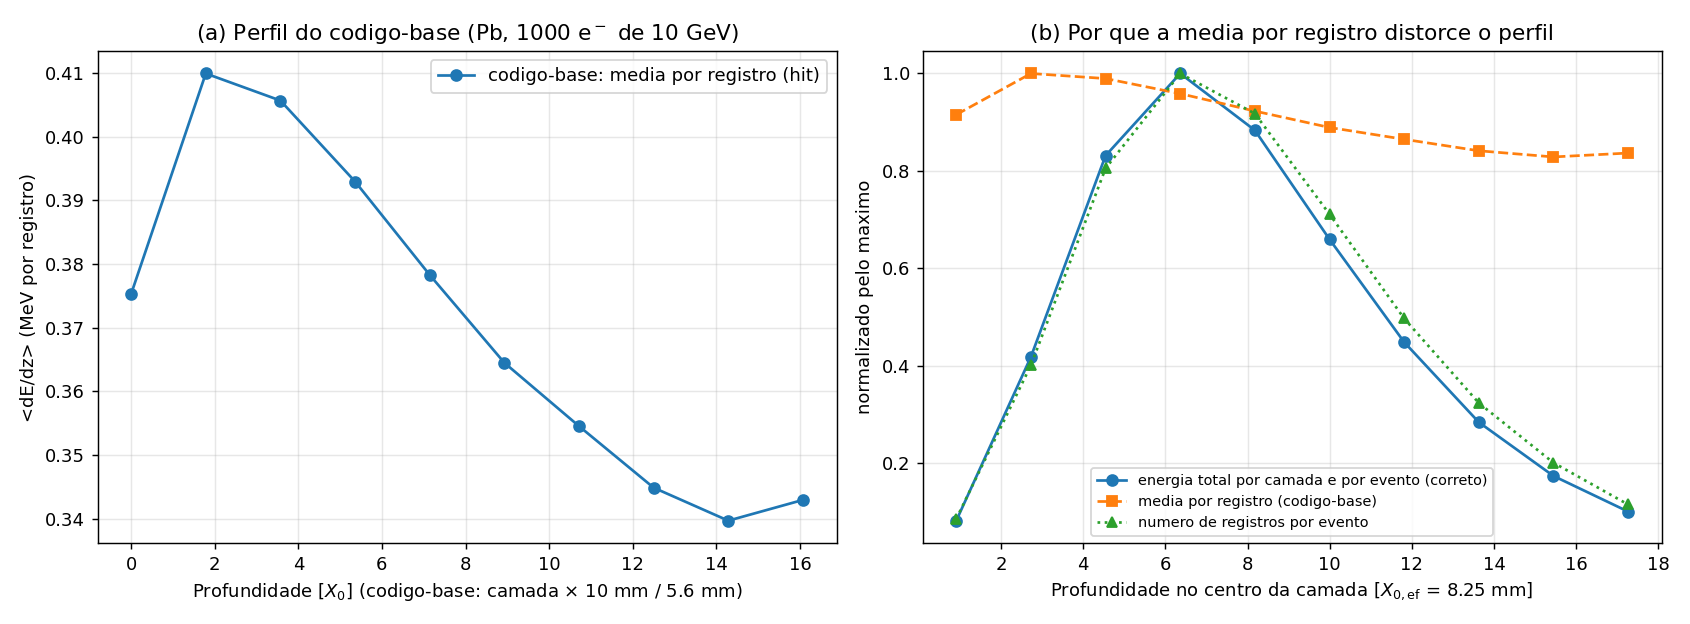
\includegraphics[width=\textwidth]{perfil_codigo_base.png}
  \caption{(a) Perfil calculado como no código-base: média de $E_\text{dep}$ por registro em cada camada, profundidade
  = camada × 10~mm / 5,6~mm. (b) Comparação de forma (normalizado pelo máximo) entre a energia total por camada e por
  evento (correto), a média por registro e o número médio de registros por evento em cada camada.}
  \label{fig:base}
\end{figure}

O código-base faz \texttt{groupby('Layer')['Edep\_MeV'].mean()}, que é a energia média de \textbf{um passo} em cada
camada, e não a energia depositada na camada. A energia na camada é (número de passos) × (energia média por passo),
e quem carrega a forma do chuveiro é o \textbf{número de passos}, que cresce com o número de partículas. Dividindo
por esse número, a forma é jogada fora: na Fig.~\ref{fig:base} a média por registro varia só entre 0,34 e 0,41~MeV
(fica quase plana), enquanto a energia real varia mais de 10×. O pouco que sobra de forma reflete detalhes do
transporte (tamanho dos passos, cortes de produção, tipo e energia das partículas em cada profundidade) e não o
chuveiro. Além disso, eventos com mais passos pesam mais na média, e eventos sem nada numa camada simplesmente
não entram, em vez de contarem como zero.

A correção é somar $E_\text{dep}$ por camada \textbf{dentro de cada evento} (usando o \texttt{EventID}), montar uma matriz
(eventos × camadas) com zero onde não houve deposição, e só então calcular a média e o desvio padrão entre os eventos.
As barras de erro da média são $\sigma/\sqrt{N}$; o desvio padrão (flutuação evento a evento) também é mostrado.

\subsection{(c) Conversão para unidades de $X_0$}

O código-base usa 10~mm por camada, mas \textbf{cada camada tem 15~mm} (10~mm de Pb + 5~mm de LAr). Ele também
usa o índice da camada como profundidade (a camada 0 em $t=0$), em vez do centro da camada.

Num calorímetro de amostragem o chuveiro atravessa materiais alternados, e o que importa é a quantidade total de
material em unidades de $X_0$. Para uma camada de espessura $d = \sum_j d_j$, o \textbf{comprimento de radiação
efetivo} é
\[
  \frac{1}{X_0^\text{ef}} = \sum_j \frac{f_j}{X_{0,j}}, \qquad f_j = \frac{d_j}{d}
  \quad\Rightarrow\quad
  X_0^\text{ef} = \frac{15~\text{mm}}{10/5{,}613 + 5/140{,}6} = 8{,}25~\text{mm}
\]
(o mesmo vale com frações de massa e $X_0$ em g/cm$^2$). Cada camada tem $1{,}817\,X_0$, e o calorímetro $18{,}2\,X_0$.
A conversão que eu proponho é $t_i = (i + \tfrac12)\, d / X_0^\text{ef}$ (centro da camada), com $dE/dt = E_i / (d/X_0^\text{ef})$.

No chumbo, o código-base dá $10/5{,}6 = 1{,}786\,X_0$ por camada, só 1,7\% abaixo. Isso é coincidência: ele erra a
espessura da camada, mas como só usa o $X_0$ do chumbo, as duas coisas quase se cancelam (o LAr contribui só
0,036~$X_0$). Com água o mesmo raciocínio erra feio: $10/361 = 0{,}028\,X_0$ por camada, contra o correto de
$0{,}063\,X_0$ (\textbf{$-56\%$}), porque aí o LAr tem mais $X_0$ que a água.

\subsection{(d) Ajuste}

\begin{figure}[H]
  \centering
  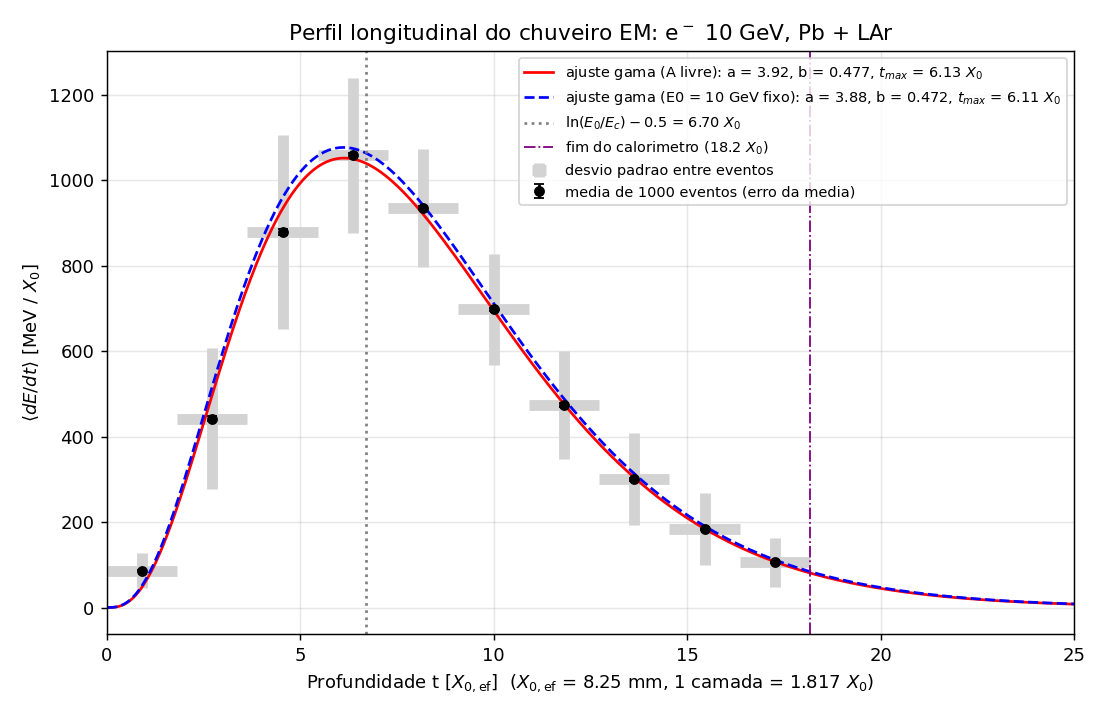
\includegraphics[width=0.85\textwidth]{perfil_longitudinal_Pb.png}
  \caption{Perfil longitudinal médio de 1000 e$^-$ de 10 GeV (Pb/LAr), em unidades de $X_0^\text{ef}$. Pontos: média
  (barra preta = erro da média; barra cinza vertical = desvio padrão entre eventos; barra horizontal = largura da
  camada). Curvas: ajuste da Eq.~(2) do enunciado.}
  \label{fig:perfil}
\end{figure}

Como cada camada tem $1{,}8\,X_0$, avaliar $dE/dt$ só no centro seria grosseiro. Ajustei a \textbf{integral} da Eq.~(2)
em cada camada, $E_i = A\,[P(a, b\,t_{i+1}) - P(a, b\,t_i)]$ ($P$ = função gama incompleta regularizada), com
\texttt{curve\_fit} e os erros da média como incerteza:

\begin{table}[H]
\centering
\begin{tabular}{lccccc}
\toprule
ajuste & $A$ (MeV) & $a$ & $b$ & $t_\text{max} = (a-1)/b$ & $\chi^2/\text{ndof}$ \\
\midrule
$A$ livre & $9727 \pm 25$ & $3{,}925 \pm 0{,}016$ & $0{,}477 \pm 0{,}002$ & $6{,}13 \pm 0{,}01\,X_0$ & 287,7/7 \\
$A = E_0 = 10$ GeV fixo & 10000 & $3{,}885 \pm 0{,}015$ & $0{,}472 \pm 0{,}002$ & $6{,}11 \pm 0{,}01\,X_0$ & 410,3/8 \\
\bottomrule
\end{tabular}
\end{table}

A estimativa da Eq.~(1) é $t_\text{max} = \ln(10000/7{,}4) - 0{,}5 = 6{,}70\,X_0$, cerca de $0{,}6\,X_0$ (9\%) acima do
ajuste. Isso é razoável, porque a Eq.~(1) é uma estimativa simples ``de bolso''. Usando uma energia crítica efetiva do
Pb/LAr ($E_c^\text{ef} \approx 7{,}9$~MeV) ela daria 6,64, o que não explica a diferença. O valor de $b \approx 0{,}48$
está perto do típico ($b \approx 0{,}5$). O $\chi^2/\text{ndof} \approx 41$ mostra que, com 1000 eventos, os erros da
média ($\sim 1\%$) já são menores que as limitações da parametrização gama, que é uma descrição aproximada do perfil
médio. O resultado de $t_\text{max}$ quase não muda entre fixar ou não a normalização.

\subsection{(e) Contenção}

Da ntuple \texttt{B4} (por evento) e conferido somando os registros:
\begin{itemize}
  \item energia total depositada: $\mathbf{93{,}8\%}$ de $E_0$ (rms de 2,0\% entre eventos);
  \item no absorvedor (Pb): $88{,}9\%$; no meio ativo (LAr): $4{,}9\%$. A fração de amostragem é $E_\text{gap}/E_\text{tot} = 5{,}2\%$:
    só 1/19 da energia seria ``vista'' de fato num detector real;
  \item a última camada ainda recebe $1{,}9\%$ de $E_0$, e o perfil ajustado prevê que $2{,}5\%$ do chuveiro estaria
    além de $18{,}2\,X_0$ (vazamento longitudinal).
\end{itemize}

\noindent O chuveiro está \textbf{quase, mas não totalmente, contido longitudinalmente}: o máximo ($6\,X_0$) fica bem
dentro do calorímetro, mas a cauda sai pela parte de trás. Os $\approx 3{,}7\%$ que faltam além do vazamento longitudinal são
vazamento lateral (o calorímetro tem $\pm 5$~cm, ou seja, $\approx 2{,}3\,R_M^\text{ef}$, com $R_M^\text{ef} \approx 21{,}2~\text{MeV}\,X_0^\text{ef}/E_c^\text{ef} \approx 22$~mm)
e partículas retroespalhadas pela face de entrada.

\noindent Com mais camadas, pelo perfil ajustado: 12 camadas ($21{,}8\,X_0$) deixariam escapar 0,7\%, 15 camadas
($27\,X_0$) 0,1\% e 20 camadas, praticamente nada. Para 99\% de contenção longitudinal seriam $\approx 21\,X_0$ (12 camadas). Mais
camadas também diminuem a flutuação causada pelo vazamento, o que melhora a resolução, mas não resolvem o vazamento lateral
(para isso é preciso aumentar \texttt{calorSizeXY}) e deixam o detector maior e mais caro.

\subsection{(f) Comparação com a água}

\begin{figure}[H]
  \centering
  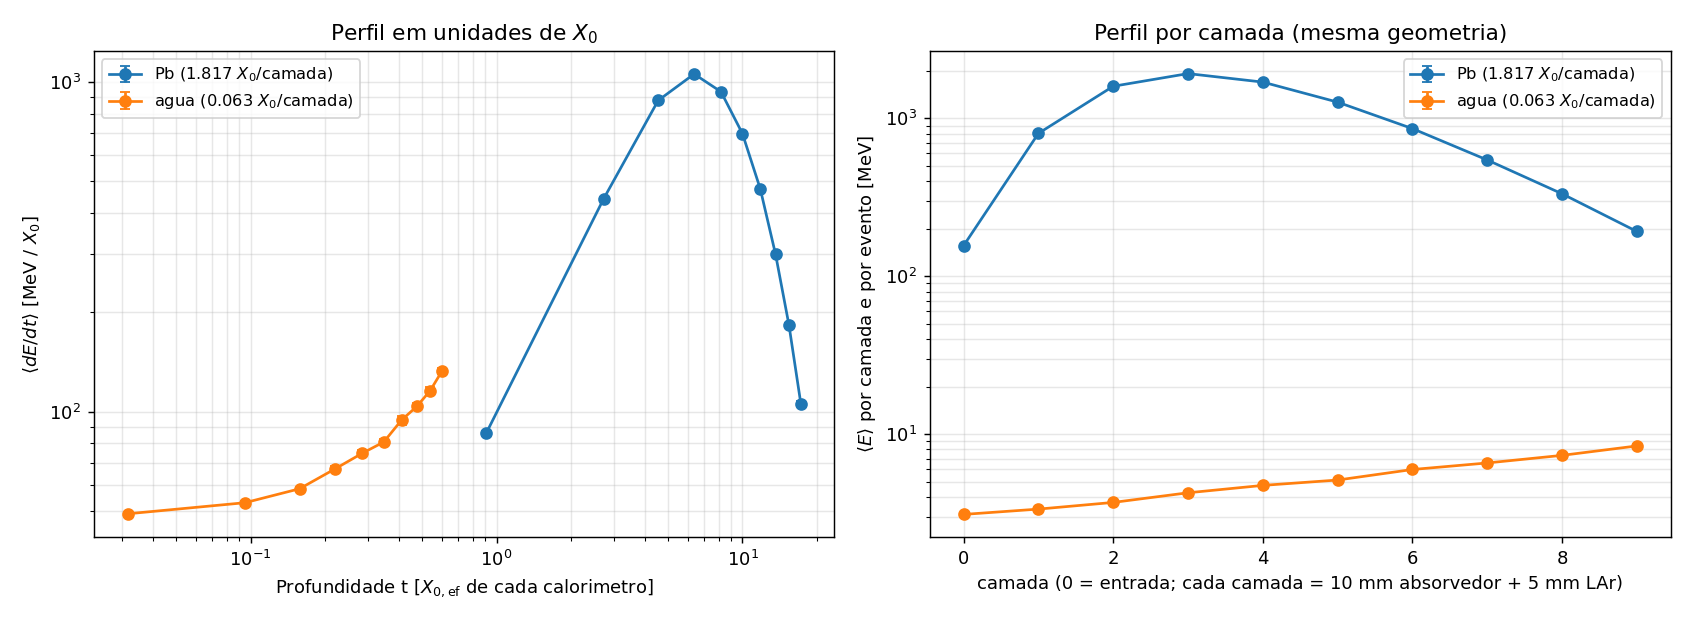
\includegraphics[width=\textwidth]{perfil_Pb_vs_agua.png}
  \caption{Perfis com absorvedor de chumbo e de água. Esquerda: $dE/dt$ em função da profundidade em $X_0^\text{ef}$ de
  cada calorímetro (escalas log). Direita: energia média por camada e por evento (mesma geometria).}
\end{figure}

Com água, $X_0^\text{ef} = 15/(10/360{,}8 + 5/140{,}6) = 237$~mm (e não os 361~mm da água pura, pelo mesmo motivo do
item (c)). O calorímetro inteiro tem só $0{,}63\,X_0$ e a figura mostra apenas o \textbf{começo} de um chuveiro: a
energia por camada cresce devagar, de 3 para 8~MeV, porque o elétron começa a irradiar e alguns fótons convertem.
Não há máximo, e não faz sentido ajustar a Eq.~(2): o máximo estaria em $\sim 6\,X_0$, quase 1,5~m de água/LAr. Só
$0{,}5\%$ da energia fica no calorímetro (0,33\% na água e 0,20\% no LAr; fração de amostragem de 37\%, porque agora o
LAr é até mais denso que a água e deposita por ionização um pouco mais por mm: 0,40 contra 0,34~MeV/mm). Em unidades de $X_0$ os dois perfis se ``encaixam'': a água cobre só
o trecho $t < 0{,}63$ que, no chumbo, fica todo dentro da primeira camada.

%=====================================================================
\section{Conclusões}
%=====================================================================

\begin{itemize}
  \item O B4a é um calorímetro EM de amostragem Pb/LAr com $18\,X_0$, mas só $0{,}6\,\lambda_I$: contém 94\% de um
    elétron de 10 GeV e só $\sim 14\%$ de um próton ou alfa, com flutuações muito grandes.
  \item Trocar Pb por água reduz a espessura para $0{,}63\,X_0$ e $0{,}19\,\lambda_I$: nada chuveira, tudo atravessa.
  \item Para o perfil longitudinal é essencial somar por evento antes de fazer a média. A média por registro do código-base
    perde a forma do chuveiro.
  \item A profundidade deve usar a espessura real da camada (15~mm) e o $X_0$ efetivo da mistura; no chumbo o erro
    do código-base se cancela por acaso, na água chega a 56\%.
  \item O ajuste gama dá $t_\text{max} = 6{,}13\,X_0$, perto da estimativa $\ln(E_0/E_c) - 0{,}5 = 6{,}7\,X_0$.
\end{itemize}

\begin{thebibliography}{9}
\bibitem{g4} Geant4 Collaboration, \emph{Book For Application Developers}, versão 11.4, e exemplo
  \texttt{examples/basic/B4} (\url{https://geant4.web.cern.ch}).
\bibitem{pdg} Particle Data Group, \emph{Review of Particle Physics}, seção ``Passage of particles through matter''
  (chuveiros eletromagnéticos, $X_0$, $E_c$, $R_M$), \url{https://pdg.lbl.gov}.
\bibitem{longo} E. Longo e I. Sestili, \emph{Monte Carlo calculation of photon-initiated electromagnetic showers in lead
  glass}, Nucl. Instrum. Meth. 128 (1975) 283 (parametrização gama do perfil longitudinal).
\end{thebibliography}

\end{document}
